\documentclass[submit]{harvardml}

\course{CS181-S22}
\assignment{Assignment \#1}
\duedate{7:59pm ET, February 4, 2022} 

\usepackage[OT1]{fontenc}
\usepackage[colorlinks,citecolor=blue,urlcolor=blue]{hyperref}
\usepackage[pdftex]{graphicx}
\usepackage{graphicx}
\usepackage{caption}
\usepackage{fullpage}
\usepackage{soul}
\usepackage{amsmath}
\usepackage{amssymb}
\usepackage{color}
\usepackage{todonotes}
\usepackage{listings}
\usepackage{common}
\usepackage{framed}

\usepackage{subcaption}

\usepackage[mmddyyyy,hhmmss]{datetime}

\definecolor{verbgray}{gray}{0.9}

\lstnewenvironment{csv}{
  \lstset{backgroundcolor=\color{verbgray},
  frame=single,
  framerule=0pt,
  basicstyle=\ttfamily,
  columns=fullflexible}}{}
 
\newcommand{\TODO}{{\color{red}TODO }}
\newcommand{\solution}{{\textbf{Solution }}}

\begin{document}
\begin{center}
{\Large Homework 1: Regression}\\
\end{center}

\subsection*{Introduction}
This homework is on different forms of linear regression and focuses
on loss functions, optimizers, and regularization. Linear regression
will be one of the few models that we see that has an analytical
solution.  These problems focus on deriving these solutions and
exploring their properties.

If you find that you are having trouble with the first couple
problems, we recommend going over the fundamentals of linear algebra
and matrix calculus (see links on website).  The relevant parts of the
\href{https://github.com/harvard-ml-courses/cs181-textbook/blob/master/Textbook.pdf}{cs181-textbook notes are Sections 2.1 - 2.7}.  We strongly recommend
reading the textbook before beginning the homework.

    We also encourage you to first read the \href{http://users.isr.ist.utl.pt/~wurmd/Livros/school/Bishop\%20-\%20Pattern\%20Recognition\%20And\%20Machine\%20Learning\%20-\%20Springer\%20\%202006.pdf}{Bishop textbook}, particularly:
Section 2.3 (Properties of Gaussian Distributions), Section 3.1
(Linear Basis Regression), and Section 3.3 (Bayesian Linear
Regression). (Note that our notation is slightly different but the
underlying mathematics remains the same!).

\textbf{Please type your solutions after the corresponding problems using this
\LaTeX\ template, and start each problem on a new page.} You may find
the following introductory resources on \LaTeX\ useful: 
\href{http://www.mjdenny.com/workshops/LaTeX_Intro.pdf}{\LaTeX\ Basics} 
and \href{https://www.overleaf.com/learn/latex/Free_online_introduction_to_LaTeX_(part_1)}{\LaTeX\ tutorial with exercises in Overleaf}

Homeworks will be submitted through Gradescope. You will be added to
the course Gradescope once you join the course Canvas page. If you
haven't received an invitation, contact the course staff through Ed.

\textbf{Please submit the writeup PDF to the Gradescope assignment
  `HW1'.} Remember to assign pages for each question.

\textbf{Please submit your \LaTeX file and code files to the
  Gradescope assignment `HW1 - Supplemental'.} Your files should be
named in the same way as we provide them in the repository,
e.g. \texttt{T1\_P1.py}, etc.


%%%%%%%%%%%%%%%%%%%%%%%%%%%%%%%%%%%%%%%%%%%%%
% Problem 1
%%%%%%%%%%%%%%%%%%%%%%%%%%%%%%%%%%%%%%%%%%%%%

\begin{problem}[Optimizing a Kernel, 15pts]

Kernel-based regression techniques are similar to nearest-neighbor
regressors: rather than fit a parametric model, they predict values
for new data points by interpolating values from existing points in
the training set.  In this problem, we will consider a kernel-based
regressor of the form:
\begin{equation*}
  f(x^*) = \sum_{n} K(x_n,x^*) y_n 
\end{equation*}
where $(x_n,y_n)$ are the training data points, and $K(x,x')$ is a
kernel function that defines the similarity between two inputs $x$ and
$x'$. Assume that each $x_i$ is represented as a column vector, i.e. a
$D$ by 1 vector where $D$ is the number of features for each data
point. A popular choice of kernel is a function that decays as the
distance between the two points increases, such as
\begin{equation*}
  K(x,x') = \exp\left(\frac{-||x-x'||^2_2}{\tau}\right) = \exp\left(\frac{-(x-x')^T (x-x')}{\tau} \right) 
\end{equation*}
where $\tau$ represents the square of the lengthscale (a scalar value).  In this
problem, we will consider optimizing what that (squared) lengthscale
should be.

\begin{enumerate}

\item Let $\{(x_n,y_n)\}_{n=1}^N$ be our training data set.  Suppose
  we are interested in minimizing the residual sum of squares.  Write
  down this loss over the training data $\mcL(W)$ as a function of $\tau$.

  Important: When computing the prediction $f(x_i)$ for a point $x_i$
  in the training set, carefully consider for which points $x'$ you should be including
  the term $K(x_i,x')$ in the sum.

\item Take the derivative of the loss function with respect to $\tau$.
\end{enumerate}

\end{problem}

\begin{enumerate}
	\item The least squares loss over the training data is
	$$\mcL(W) = \sum_{n=1}^N \left(y_n - f(x_n)\right)^2.$$
	Substituting $f(x_n)$ with its definition, including all terms $K(x_n, x_i)$ in the sum except when $n = i$, to prevent leakage from using $y_n$ to predict $f(x_n)$:
	$$\mcL(W) = \sum_{n=1}^N \left(y_n - \sum_{i \neq n} K(x_n, x_i)y_i\right)^2
	= \sum_{n=1}^N \left(y_n - \sum_{i \neq n} \exp\left(\frac{-||x-x'||^2_2}{\tau}\right)y_i\right)^2.$$
	
	\item Differentiating,
	\begin{align*}
		\frac{d}{d\tau} \mcL(W) &= \frac{d}{d\tau} \sum_{n=1}^N \left(y_n - \sum_{i \neq n} \exp\left(\frac{-||x-x'||^2_2}{\tau}\right)y_i\right)^2 \\
		&= 2 \sum_{n=1}^N \left(y_n - \sum_{i \neq n} \exp\left(\frac{-||x-x'||^2_2}{\tau}\right)y_i\right) \cdot \sum_{i \neq n} \left(\frac{-||x-x'||^2_2}{\tau^2}\right) \exp\left(\frac{-||x-x'||^2_2}{\tau}\right)y_i.
	\end{align*}
	
	
\end{enumerate}

\newpage

\begin{framed}
\noindent\textbf{Problem 1} (cont.)\\

\begin{enumerate}
\setcounter{enumi}{2}
\item Consider the following data set:
\begin{csv}
  x , y
  0 , 0
  1 , 0.5
  2 , 1
  3 , 2
  4 , 1
  6 , 1.5
  8 , 0.5 
\end{csv}
And the following lengthscales: $\tau=.01$, $\tau=2$, and $\tau=100$.

Write some Python code to compute the loss with respect to each kernel
for the dataset provided above. Which lengthscale does best?  
For this problem, you can use our staff \textbf{script to compare your
  code to a set of staff-written test cases.} This requires, however,
that you use the structure of the starter code provided in
\texttt{T1\_P1.py}. More specific instructions can be found at the top
of the file \texttt{T1\_P1\_Testcases.py}. You may run the test cases
in the command-line using \texttt{python T1\_P1\_TestCases.py}.
\textbf{Note that our set of test cases is not comprehensive: just
  because you pass does not mean your solution is correct! We strongly
  encourage you to write your own test cases and read more about ours
  in the comments of the Python script.}
  
\item Plot the function $(x^*, f(x^*))$ for each of the
  lengthscales above.  You will plot $x^*$ on the x-axis and the
  prediction $f(x^*)$ on the y-axis.  For the test inputs $x^*$, you
  should use an even grid of spacing of $0.1$ between $x^* = 0$ and
  $x^* = 12$.  (Note: it is possible that a test input $x^*$ lands
  right on top of one of the training inputs above.  You can still use
  the formula!) 

  Initial impressions: Briefly describe what happens in each of the
  three cases.  Is what you see consistent with the which lengthscale
  appeared to be numerically best above?  Describe why or why not.

\item Bonus: Code up a gradient descent to optimize the kernel for the
  data set above.
  Start your gradient descent from $\tau=2$. Report on what you
  find.\\\\

  Note: Gradient descent is discussed in Section 3.4 of the
  cs181-textbook notes and Section 5.2.4 of Bishop, and will be
  covered later in the course!

\end{enumerate}
  
\end{framed}

\begin{enumerate}
	\setcounter{enumi}{2}
	\item The losses are \\
	\texttt{
	Loss for tau = 0.01: 8.75 \\
	Loss for tau = 2: 3.305016494565789 \\
	Loss for tau = 100: 120.35919342230957}. \\
	The lengthscale that does best is $\tau = 2$, which minimizes the loss over the three lengthscales tested.

	\item 
	
	\begin{figure}[h]
		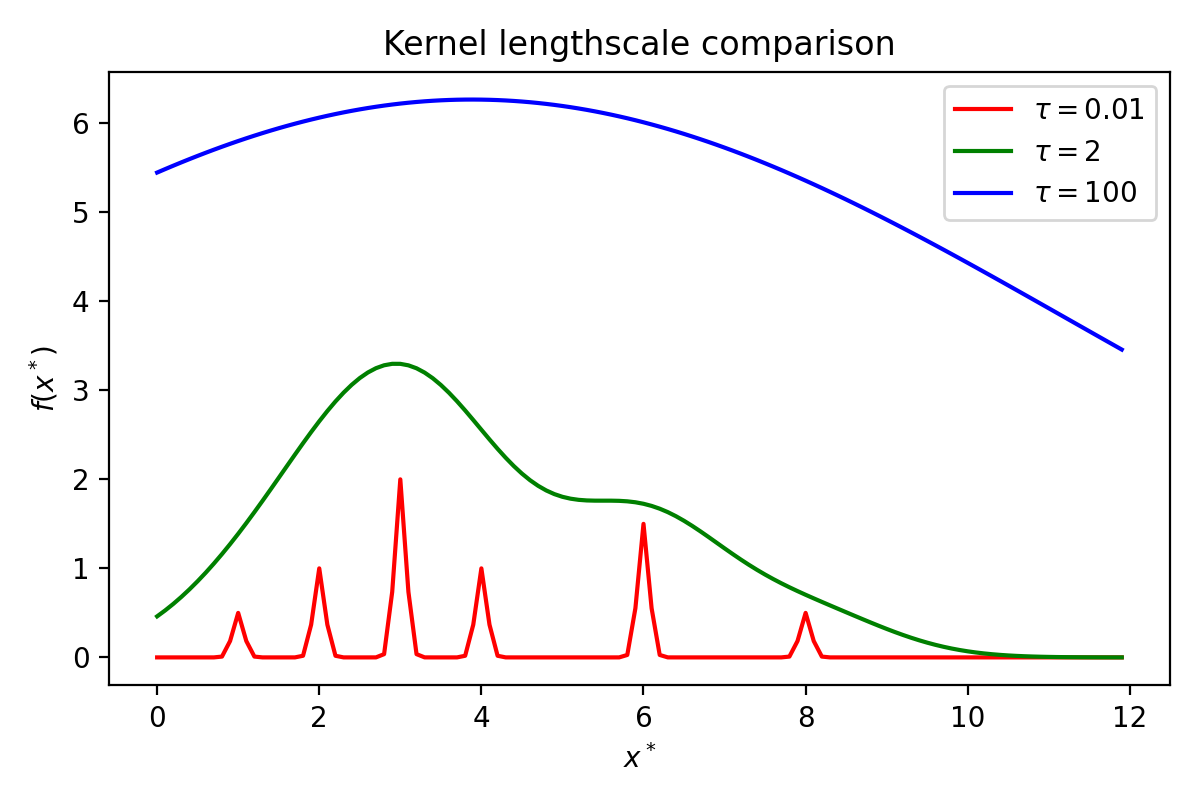
\includegraphics{T1_P1_plot}
	\end{figure}

	The plots demonstrate that as $\tau$ increases, values farther away in the training set are weighted higher relative to closer values. When $\tau = 0.01$, $f(x^*)$ has very sharp peaks around the training values and is zero everywhere else, meaning that predictions are highly based on close values. When $\tau = 2$, $f(x^*)$ is smoother, because it lends a fair amount of weight to close values and less to far values. When $\tau = 100$, $f(x^*)$ is extremely smooth because it weighs all values similarly, so much so that nuances in the training set are lost.
	
	This is consistent with $\tau=2$ being the numerically best of the three lengthscales, since the corresponding $f(x^*)$ is curvy enough to follow the trends in the training data, while being smooth enough to approximate points in between those in the training data.

	\item Bonus

\end{enumerate}


\newpage

%%%%%%%%%%%%%%%%%%%%%%%%%%%%%%%%%%%%%%%%%%%%%
% Problem 2
%%%%%%%%%%%%%%%%%%%%%%%%%%%%%%%%%%%%%%%%%%%%%

\begin{problem}[Kernels and kNN, 10pts]

Now, let us compare the kernel-based approach to an approach based on
nearest-neighbors.  Recall that kNN uses a predictor of the form
  \begin{equation*}
    f(x^*) = \frac{1}{k} \sum_n y_n \mathbb{I}(x_n \texttt{ is one of k-closest to } x^*)
  \end{equation*}

\noindent where $\mathbb{I}$ is an indicator variable. For this problem, you will use the \textbf{same dataset and kernel as in Problem 1}.


For this problem, you can use our staff \textbf{script to compare your code to a set of staff-written test cases.} This requires, however, that you use the structure of the starter code provided in \texttt{T1\_P2.py}. More specific instructions can be found at the top of the file \texttt{T1\_P2\_Testcases.py}. You may run the test cases in the command-line using \texttt{python T1\_P2\_TestCases.py}.
\textbf{Note that our set of test cases is not comprehensive: just because you pass does not mean your solution is correct! We strongly encourage you to write your own test cases and read more about ours in the comments of the Python script.}

\vspace{0.5cm}
\noindent\emph{Make sure to include all required plots in your PDF.}


\begin{enumerate}

\item Implement kNN for $k=\{1, 3, N-1\}$ where N is the size of the dataset, then plot the results for each $k$. To find the distance between points, use the kernel function from Problem 1 with lengthscale $\tau=1$. 

As before, you will plot $x^*$ on the x-axis and the prediction $f(x^*)$ on the y-axis.  For the test inputs $x^*$, you should use an even grid of spacing of $0.1$ between $x^* = 0$ and $x^* = 12$.  (Like in Problem 1, if a test point lies on top of a training input, use the formula without excluding that training input.)
  
  You may choose to use some starter Python code to create your plots
  provided in \verb|T1_P2.py|.  Please \textbf{write your own
    implementation of kNN} for full credit.  Do not use external
  libraries to find nearest neighbors.
  
\item Describe what you see: What is the behavior of the functions in
  these three plots?  How does it compare to the behavior of the
  functions in the three plots from Problem 1?  Are there situations
  in which kNN and kernel-based regression interpolate similarly?
  Extrapolate similarly?  Based on what you see, do you believe there
  exist some values of $k$ and $\tau$ for which the kNN and kernel-based regressors produce the exact same classifier (ie. given \textit{any} point $x$, the two regressors will produce the same prediction $f(x)$)? Explain your answer.
  
\item Why did we not vary $\tau$ for the kNN approach?

\end{enumerate}

\end{problem}

\begin{enumerate}
	\item See Figure \ref{fig:kNN}.
	
	\begin{figure}[h]
			\centering
			\begin{subfigure}[b]{0.475\textwidth}
				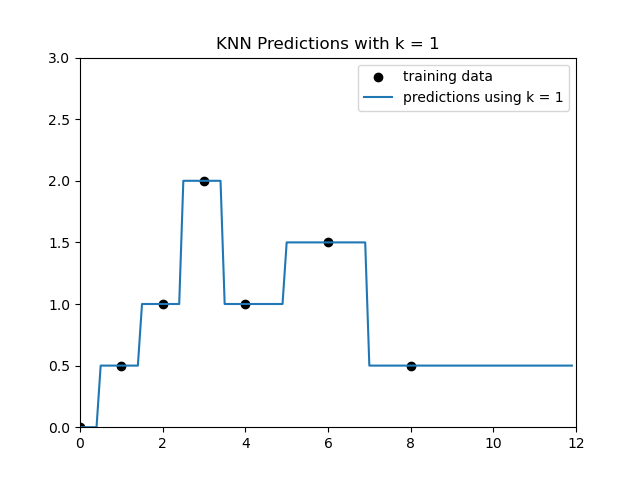
\includegraphics[width=\textwidth]{k1}
			\end{subfigure}
		 	\hfill
			\begin{subfigure}[b]{0.475\textwidth}
				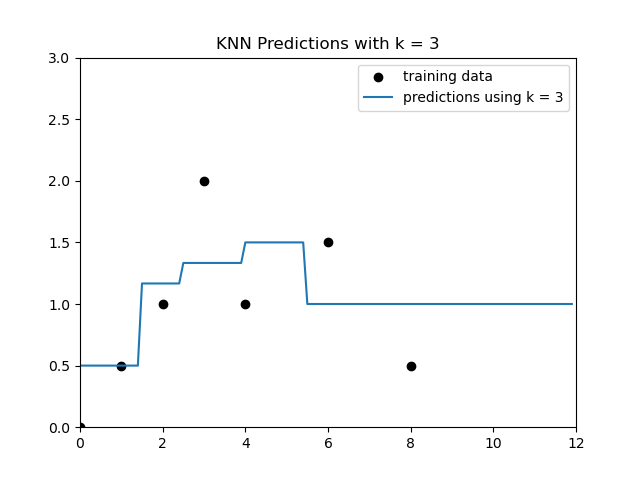
\includegraphics[width=\textwidth]{k3}
			\end{subfigure}
			\hfill
			\vskip\baselineskip
			\begin{subfigure}[b]{0.475\textwidth}
				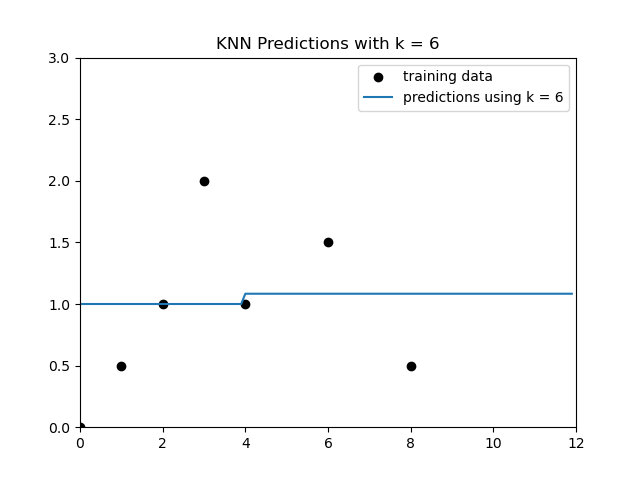
\includegraphics[width=\textwidth]{k6}
			\end{subfigure}
			\caption{KNN Predictions}
			\label{fig:kNN}
	\end{figure}

	
	\item All of the kNN functions are  step functions comprised of flat sections, where points in a given range have the same $k$ nearest neighbors, and rapid jumps, where one of the nearest neighbors changes and the value of $f(x^*)$ changes accordingly. As with $\tau$ in kernel-based regression, lower values of $k$ are more influenced by local training data points, while higher values of $k$ are more globally influenced. Also as with kernel-based regression, the first parameter tested seems to overfit the data, the second fits relatively well, and the underfits the data. Interpolation is somewhat similar between kernel-based regression and kNN, but extrapolation is very different. Because all $x^*$ greater than the greatest $x_n$ in the training set have the same $k$ nearest neighbors, they all map to the same $f(x^*)$, and likewise with $x^*$ smaller than the smallest $x_n$. This means kNN extrapolates quite poorly, in contrast to kernel-based regression with appropriate values of $\tau$, which smooths off convincingly as the data trends down when $x^*$ increases.
	
	Based on this, it does not seem as though there are $k$ and $\tau$ such that the kNN and kernel-based regressors produce the exact same classifier, since kernel-based regression is ``smooth" and the kNN functions are step functions, regardless of $k$ and $\tau$. Consequently, the approaches extrapolate differently. A possible exception might be $k \geq N$ and very large values of $\tau$, both of which effectively map all points to the average of the training data $y$ values, but this would still be an approximate match.
	
	\item The value of $\tau$ does not matter for the kNN approach, as long as it is positive, because the values of $K(x_n, x^*)$ change depending on $\tau$, but the relative orderings of the $k$ nearest neighbors will be the same. The means that the same $k$ nearest neighbors are selected regardless of $\tau$, and thus the predicted values will be the same.
	
\end{enumerate}

\newpage 

%%%%%%%%%%%%%%%%%%%%%%%%%%%%%%%%%%%%%%%%%%%%%
% Problem 3
%%%%%%%%%%%%%%%%%%%%%%%%%%%%%%%%%%%%%%%%%%%%%

\begin{problem}[Deriving Linear Regression, 10pts]

  The solution for the least squares linear regressions ``looks'' kind
  of like a ratio of covariance and variance terms.  In this problem,
  we will make that connection more explicit. \\

  \noindent Let us assume that our data are tuples of scalars $(x,y)$ that are
  described by some joint distribution $p(x,y)$.  For clarification, the joint distribution $p(x,y)$ is just another way of saying the ``joint PDF'' $f(x,y)$, which may be more familiar to those who have taken Stat 110, or equivalent. \\
  
  \noindent We will consider the process of fitting these data from this distribution with the best linear model
  possible, that is a linear model of the form $\hat{y} = wx$ that
  minimizes the expected squared loss $E_{x,y}[ ( y - \hat{y} )^2
  ]$.\\

\noindent \emph{Notes:} The notation $E_{x, y}$ indicates an
expectation taken over the joint distribution $p(x,y)$.  Since $x$ and
$y$ are scalars, $w$ is also a scalar.
  
  \begin{enumerate}

  \item Derive an expression for the optimal $w$, that is, the $w$
    that minimizes the expected squared loss above.  You should leave
    your answer in terms of moments of the distribution, e.g. terms
    like $E_x[x]$, $E_x[x^2]$, $E_y[y]$, $E_y[y^2]$, $E_{x,y}[xy]$
    etc.

\item Provide unbiased and consistent formulas to estimate $E_{x, y}[yx]$
 and $E_x[x^2]$ given observed data $\{(x_n,y_n)\}_{n=1}^N$.

\item In general, moment terms like $E_{x, y}[yx]$, $E_{x, y}[x^2]$,
  $E_{x, y}[yx^3]$, $E_{x, y}[\frac{x}{y}]$, etc. can easily be
  estimated from the data (like you did above).  If you substitute in
  these empirical moments, how does your expression for the optimal
  $w^*$ in this problem compare with the optimal $w^*$ that we see in
  Section 2.6 of the cs181-textbook?

\item Many common probabilistic linear regression models assume that
  variables x and y are jointly Gaussian.  Did any of your above
  derivations rely on the assumption that x and y are jointly
  Gaussian?  Why or why not?
    
\end{enumerate}

\end{problem}

\begin{enumerate}
	\item The expected squared loss expands to
	\begin{align*}
	E_{x,y}[(y-\hat{y})^2] &= E_{x,y}[(y-wx)^2]  \\
	&= E_{x,y}[y^2 - 2wyx + w^2x^2] \\
	&= E_{x,y}[y^2] - 2wE_{x,y}[yx] + w^2E_{x,y}[x^2].
	\end{align*}
	Differentiating with respect to $w$ gives
	$$-2E_{x, y}[yx] + 2wE_{x, y}[x^2].$$
	To optimize $w$, set equal to zero and solve, giving
	$$w^* = \frac{E_{x,y}[yx]}{E_{x,y}[x^2]} = \frac{E_{x,y}[yx]}{E_{x}[x^2]}.$$
	
	\item The moments can be estimated by appropriately manipulating and averaging the observed quantities: $$E_{x,y}[yx] \approx \frac1N \sum_{i=1}^N y_i x_i$$
	$$E_{x}[x^2] \approx \frac1N \sum_{i=1}^N x_i^2.$$
	These formulas are unbiased and consistent because they approach the true expected values as more data is provided.
	
	\item Substituting in the empiricial moments and treating the scalars as $(1 \times 1)$ vectors,
	$$w^* \approx \frac{\frac1N\sum_{i=1}^N y_i x_i}{\frac1N\sum_{i=1}^N x_i^2} = \frac{\sum_{i=1}^N y_i x_i}{\sum_{i=1}^N x_i^2} = \frac{x^Ty}{x^Tx} = (x^Tx)^{-1}x^Ty,$$
	which is equal to the optimal $w^*$ from the textbook in the $D = 1$ case.
	
	\item No, none of my above derivations relied on the assumption that $x$ and $y$ are jointly Gaussian, because they did not use any special properties or identities particular to jointly Gaussian distributions. The expressions are comprised of moments, which can come from any distribution.

\end{enumerate}

%%%%%%%%%%%%%%%%%%%%%%%%%%%%%%%%%%%%%%%%%%%%%
% Problem 4
%%%%%%%%%%%%%%%%%%%%%%%%%%%%%%%%%%%%%%%%%%%%%

\begin{problem}[Modeling Changes in Republicans and Sunspots, 15pts]
  
 The objective of this problem is to learn about linear regression
 with basis functions by modeling the number of Republicans in the
 Senate. The file \verb|data/year-sunspots-republicans.csv| contains the
 data you will use for this problem.  It has three columns.  The first
 one is an integer that indicates the year.  The second is the number
 of Sunspots observed in that year.  The third is the number of Republicans in the Senate for that year.
 The data file looks like this:
 \begin{csv}
Year,Sunspot_Count,Republican_Count
1960,112.3,36
1962,37.6,34
1964,10.2,32
1966,47.0,36
\end{csv}

You can see scatterplots of the data in the figures below.  The horizontal axis is the Year, and the vertical axis is the Number of Republicans and the Number of Sunspots, respectively.

\begin{center}
\includegraphics[width=.5\textwidth]{data/year-republicans}
\end{center}

\begin{center}
\includegraphics[width=.5\textwidth]{data/year-sunspots}
\end{center}

(Data Source: \url{http://www.realclimate.org/data/senators_sunspots.txt})\\
\vspace{-5mm}


\vspace{0.5cm}
\noindent\emph{Make sure to include all required plots in your PDF.}

\begin{enumerate}

\item In this problem you will implement ordinary least squares
  regression using 4 different basis functions for \textbf{Year
    (x-axis)} v. \textbf{Number of Republicans in the Senate
    (y-axis)}. Some starter Python code that implements simple linear
  regression is provided in \verb|T1_P4.py|.

  Note: The numbers in the \emph{Year} column are large (between $1960$ and $2006$), especially when raised to various powers. To avoid numerical instability due to ill-conditioned matrices in most numerical computing systems, we will scale the data first: specifically, we will scale all ``year'' inputs by subtracting $1960$ and then dividing by $40$. Similarly, to avoid numerical instability with numbers in the \emph{Sunspot\_Count} column, we will also scale the data first by dividing all ``sunspot count'' inputs by $20$. Both of these scaling procedures have already been implemented in lines $65-69$ of the starter code in \verb|T1_P4.py|. Please do \emph{not} change these lines!

First, plot the data and regression lines for each of the following sets of basis functions, and include
the generated plot as an image in your submission PDF. You will therefore make 4 total plots:
\begin{enumerate}
	\item[(a)] $\phi_j(x) = x^j$ for $j=1, \ldots, 5$\\
    ie, use basis $y = a_1 x^1 + a_2 x^2 + a_3 x^3 + a_4 x^4 + a_5 x^5$ for some constants $\{a_1, ..., a_5\}$. 
    \item[(b)] $\phi_j(x) = \exp{\frac{-(x-\mu_j)^2}{25}}$ for $\mu_j=1960, 1965, 1970, 1975, \ldots 2010$
	\item[(c)] $\phi_j(x) = \cos(x / j)$ for $j=1, \ldots, 5$
	\item[(d)] $\phi_j(x) = \cos(x / j)$ for $j=1, \ldots, 25$
\end{enumerate}
\vspace{-2mm}


{\footnotesize * Note: Please make sure to add a bias term for all your basis functions above in your implementation of the \verb|make_basis| function in \verb|T1_P4.py|.}
  
Second, for each plot include the residual sum of squares error. Submit the generated plot and residual sum-of-squares error for each basis in your LaTeX write-up.
\end{enumerate}

\end{problem}

\begin{framed}
\noindent\textbf{Problem 4} (cont.)\\
\begin{enumerate}
\setcounter{enumi}{1}
\item Repeat the same exact process as above but for \textbf{Number of Sunspots (x-axis)} v. \textbf{Number of Republicans in the Senate (y-axis)}. 
Now, however, only use data from before 1985, and only use basis functions (a), (c), and (d) -- ignore basis (b). You will therefore make 3 total plots. For each plot make sure to also include the residual sum of squares error.



Which of the three bases (a, c, d) provided the "best" fit? \textbf{Choose one}, and keep in mind the generalizability of the model. 

Given the quality of this fit, do you believe that the number of sunspots controls the number of Republicans in the senate (Yes or No)?
\end{enumerate}
\end{framed}

\begin{enumerate}
	\item
	
	\begin{figure}[h]
		\centering
		\begin{subfigure}[b]{0.475\textwidth}
			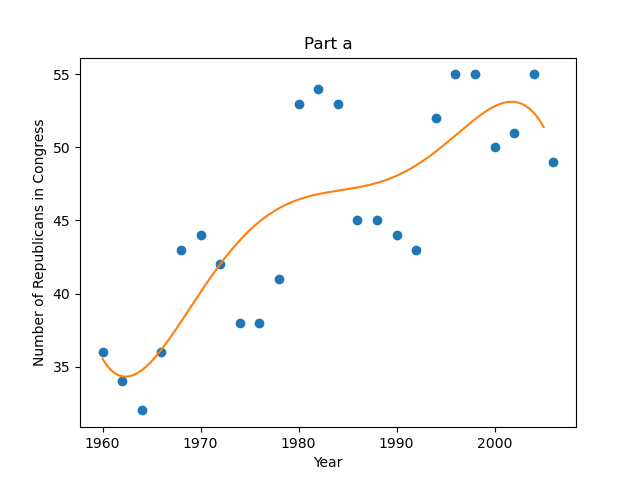
\includegraphics[width=\textwidth]{a}
		\end{subfigure}
		\hfill
		\begin{subfigure}[b]{0.475\textwidth}
			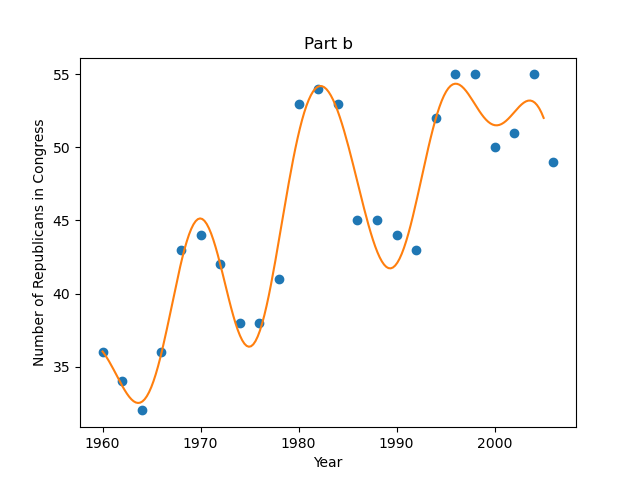
\includegraphics[width=\textwidth]{b}
		\end{subfigure}
		\hfill
		\vskip\baselineskip
		\begin{subfigure}[b]{0.475\textwidth}
			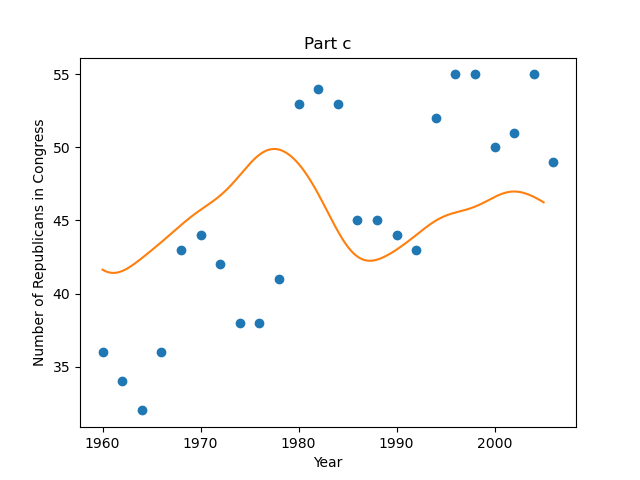
\includegraphics[width=\textwidth]{c}
		\end{subfigure}
		\hfill
		\begin{subfigure}[b]{0.475\textwidth}
			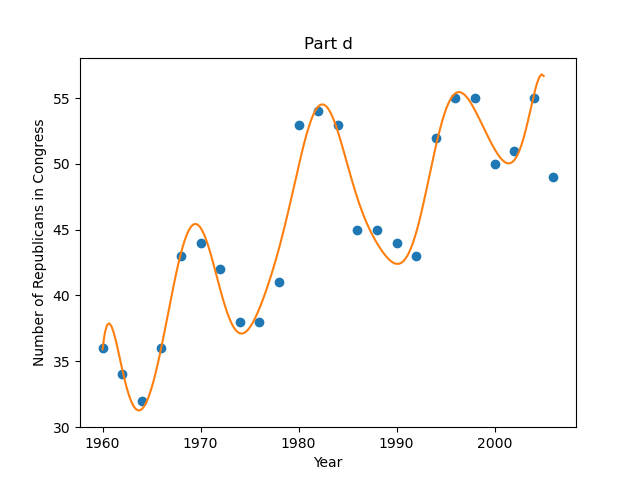
\includegraphics[width=\textwidth]{d}
		\end{subfigure}
		\caption{Year v. Republicans Bases}
		\label{fig:4.1}
	\end{figure}

	See Figure \ref{fig:4.1} for plots. The residual sum of squares errors are:
	
	\begin{center}
	\begin{tabular}{|c|c|}
		\hline
		a & 394.980 \\ \hline
		b & 54.273 \\ \hline
		c & 1082.809 \\ \hline
		d & 39.001 \\ \hline
	\end{tabular}
	\end{center}
	All of the bases did reasonably well for predicting years versus number of Republicans in the Senate, but bases b and d were clearly the best, with d being best overall due to better prediction in the most recent years. Basis c did not perform as well as d simply because it had fewer component cosine functions to work with. Basis a tended to result in a regression line in the middle of the data points, as opposed to one that oscillated to predict them more accurately.

	\item 
	
		\begin{figure}[h]
		\centering
		\begin{subfigure}[b]{0.475\textwidth}
			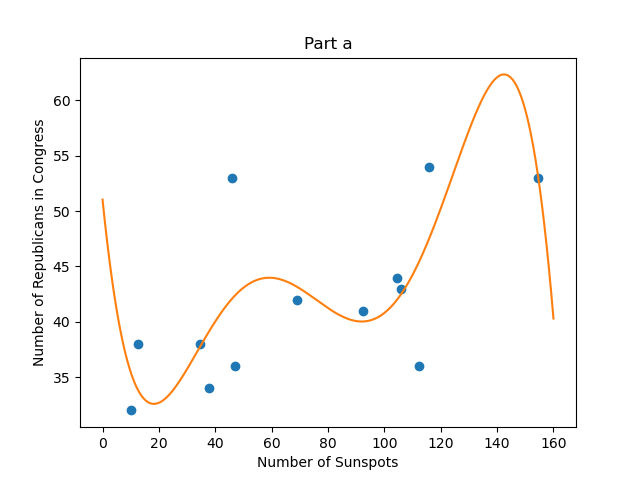
\includegraphics[width=\textwidth]{a_sunspots}
		\end{subfigure}
		\hfill
		\begin{subfigure}[b]{0.475\textwidth}
			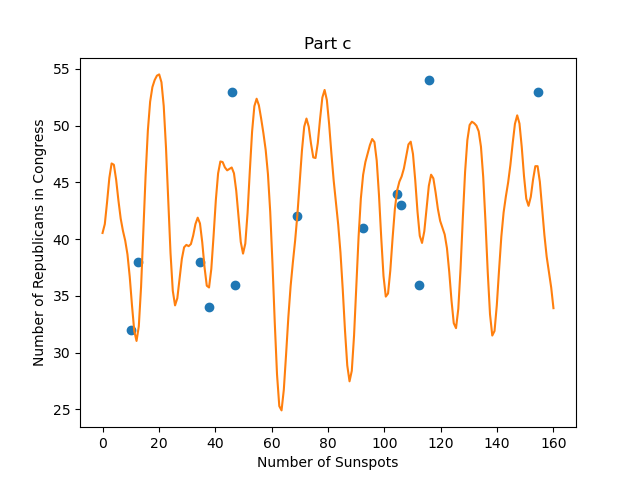
\includegraphics[width=\textwidth]{c_sunspots}
		\end{subfigure}
		\hfill
		\vskip\baselineskip
		\begin{subfigure}[b]{0.475\textwidth}
			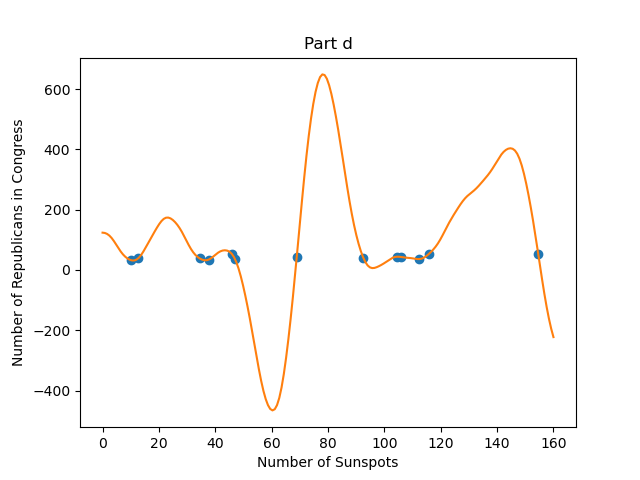
\includegraphics[width=\textwidth]{d_sunspots}
		\end{subfigure}
		\caption{Sunspots v. Republicans Bases}
		\label{fig:4.2}
	\end{figure}

	See Figure \ref{fig:4.2} for plots. The residual sum of squares errors are:

	\begin{center}
		\begin{tabular}{|c|c|}
			\hline
			a & 351.228 \\ \hline
			b & 375.107 \\ \hline
			d & 1.7054552789315644e-21 \\ \hline
		\end{tabular}
	\end{center}
	
	Basis d technically provided the best fit because it it made the residual sum of squares error basically zero. (Additionally, in the question 4.1, d provided the lowest error and the best visual fit.)
	
	However, in this question, the plot made by d is highly suspect. Even though it passes through all of the data points, it has massive peaks outside of them and also dips below zero to predict negative numbers of Republicans in the Senate, which does not make sense. Given the low quality of this fit, and the low qualities of the other bases a and c, I do not believe that the number of sunspots controls the number of Republicans in the Senate. If this were the case, I would expect at least one of the regression lines to show a clear positive (or negative) correlation between the number of sunspots and number of Republicans in the Senate, since this would be implied by causation.	

\end{enumerate}



\newpage
%%%%%%%%%%%%%%%%%%%%%%%%%%%%%%%%%%%%%%%%%%%%%
% Name and Calibration
%%%%%%%%%%%%%%%%%%%%%%%%%%%%%%%%%%%%%%%%%%%%%
\subsection*{Name}

Alex Encalada-Stuart

\subsection*{Collaborators and Resources}
Whom did you work with, and did you use any resources beyond cs181-textbook and your notes?

I did not collaborate with anyone. The CS 181 Code Crash Course was very helpful, but other than that I did not use other resources.

\subsection*{Calibration}
Approximately how long did this homework take you to complete (in hours)? 

12

\end{document}